\section{Application Security Basics}

\subsection{HTTP Basics}

HTTP ist \textbf{Zustandslos}: Der Client sendet eine Anfrage (\textbf{Request}) an den Server, welcher sie verarbeitet und anschliessend das Resultat als Antwort (\textbf{Response}) zurücksendet.\\

\begin{figure}[H]
	\centering
	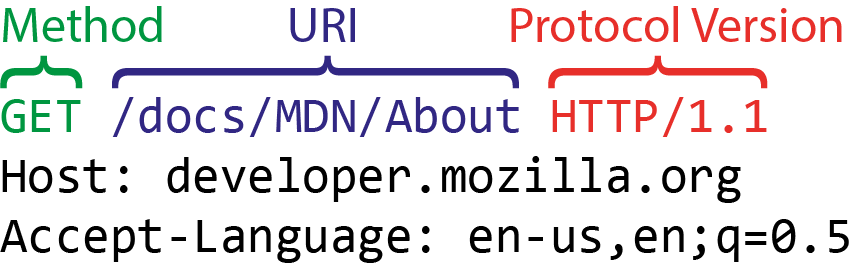
\includegraphics[width=0.38\textwidth]{./img/http-head}
	\caption{HTTP Header}
\end{figure}

Zwischen HTTP GET und POST gibt es einen wesentlichen Unterschied. Da der Server die URI in der Regel mitloggt, werden auch die \textbf{Parameter des GET-Request mitgeloggt}. Beim POST-Request geschieht dies nicht, da sich die Parameter anstatt in der URI im Body befinden. Dies ist auch bei Proxies zu beachten. Eine \textbf{Response} ist beinahe Identisch zum Request. Die erste Zeile enthält nun das Protokoll, Statuscode und Statusbeschreibung (HTTP/1.1 200 OK).

\begin{figure}[H]
	\centering
	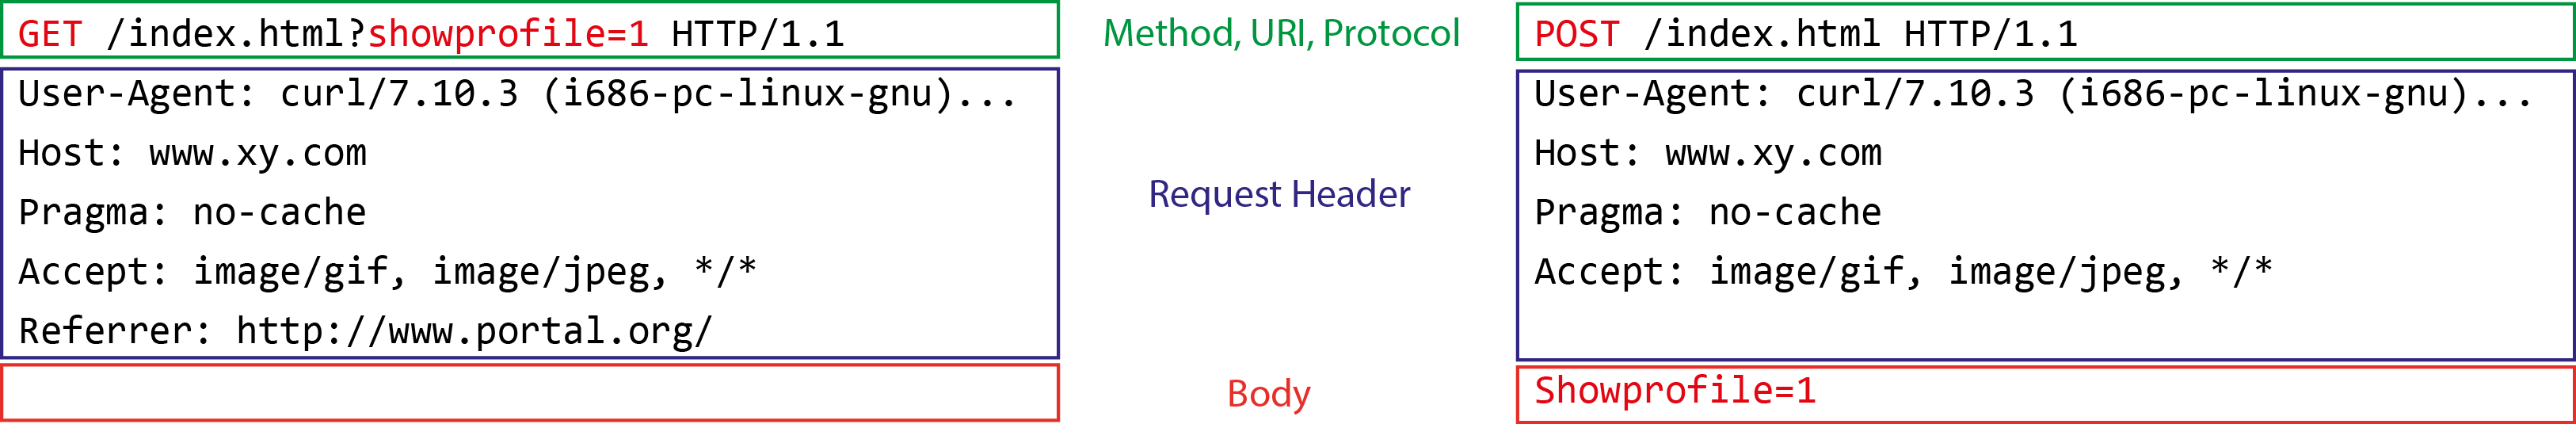
\includegraphics[width=\textwidth]{./img/http-full-request}
	\caption{Beispielrequests für GET und POST}
\end{figure}

\begin{table}[H]
	\begin{tabularx}{\textwidth}{l|X}
		\textbf{HTTP Methode} & \textbf{Verwendung}\\ \hline
		GET		& normale verwendung *\\ \hline
		POST	& übermittlung von Daten (Login, Formulare) *\\ \hline
		HEAD	& Suchmaschinen (Head of page) *\\ \hline
		PUT		& Upload von Dateien (webdav, RESTful)\\ \hline
		DELETE	& Löschen von Dateien (webdav, RESTful)\\ \hline
		OPTIONS	& Auflistung verfügbarer Methoden auf Server\\ \hline
		TRACE	& Debugging in Webserver\\ \hline
	\end{tabularx}
	\caption{Übliche HTTP Methoden (* meist verwendet)}
\end{table}


\begin{table}[H]
	\begin{tabularx}{\textwidth}{l|p{100pt}|X}
		\textbf{Statuscode} & \textbf{Nachricht} & \textbf{Bedeutung}\\ \hline
		\multicolumn{3}{c}{2xx - Erfolgreich} \\ \hline
		200 & OK & Anfrage erfolgreich bearbeitet, Ergebnis in der Antwort enthalten. \\ \hline
		\multicolumn{3}{c}{3xx - Umleitung} \\ \hline
		301 & Moved Permanently & Header "'Location: http://other-site/"' \\ \hline
		302 & Moved Temporarily & Header "'Location: http://other-site/"'; Alternativ 303 oder 307 möglich \\ \hline
		\multicolumn{3}{c}{4xx - Clientfehler} \\ \hline
		400 & Bad Request & Anfrage war fehlerhaft aufgebaut \\ \hline
		401 & Unauthorized & Authentifizierung nötig \\ \hline
		403 & Forbidden & Mangelnde Berechtigung des Clients \\ \hline
		404 & Not Found & Angeforderte Ressource nicht gefunden \\ \hline
		405 & Method Not Allowed & \\ \hline
		408 & Request Timeout & \\ \hline
		\multicolumn{3}{c}{5xx - Serverfehler} \\ \hline
		500 & Internal Server Error & Allgemeiner Serverfehler \\ \hline
		501 & Not Implemented & Funktionalität wird vom Server nicht bereitgestellt \\ \hline
		502 & Bad Gateway & Proxy hat ungültige Antwort erhalten \\ \hline
		503 & Service Unavailable & Service steht temporär nicht zur verfügung \\ \hline
	\end{tabularx}
	\caption{Übliche HTTP Statuscodes, \url{https://de.wikipedia.org/wiki/HTTP-Statuscode}}
\end{table}

\subsubsection{ZAP Inspection Proxy}
ZAP ist ein Inspection Proxy für die Analyse von Web Anwendungen. Der Proxy terminiert auch SSL-Verbindungen und verschlüsselt diese anschliessend neu. Dadurch können auch SSL-Verbindungen analysiert werden. (Dies jedoch nur ohne Fehlermeldung beim User, wenn das Proxy-CA im Browser als Trusted importiert ist, wie dies bei Unternehmens-Proxy häufig der Fall ist.)

\subsubsection{Redirect after succesful Login}
Unter diesem Namen verbirgt sich ein Pattern, um die "'\textbf{Back Button Relogin Vulnerability}"' zu adressieren. Ohne Anwendung dieses Patterns besteht die Möglichkeit, dass nach mehrmaligem Klick auf Zurück die eingegebenen Logindaten erneut an den Server übertragen werden. Bei Fehlschlag des Logins kann mittels eines gewöhnlichen \textit{200 OK} um eine erneute Eingabe gebeten werden.

\begin{figure}[H]
	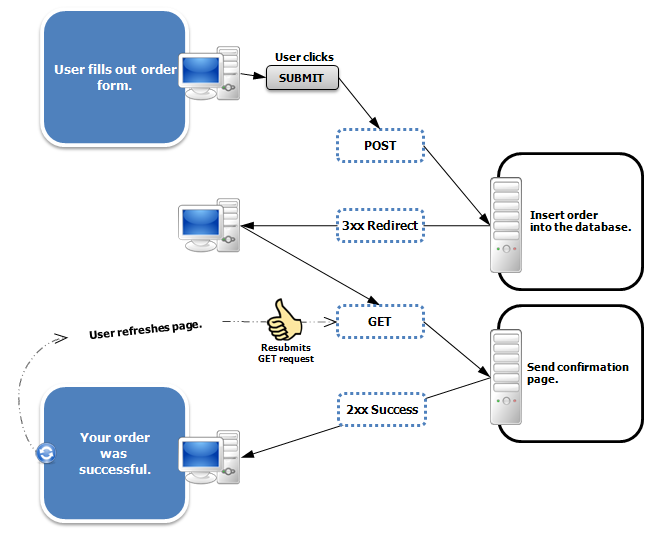
\includegraphics[width=\textwidth]{./img/PostRedirectGet_DoubleSubmitSolution}
	\caption{Redirect after succesful login}
\end{figure}

Es gibt dabei mehrere Varianten für den Redirect:
\begin{easylist}
	& Type 1 (302 Moved Temporarily) - \textbf{Browser-Memory Reset}
	&& HTTP Response Status 302
	&& HTTP Response Header "'Location: http://other-site/"'
	& Type 2 (200 OK) - \textbf{Daten in Browser-Memory gespeichert!}
	&& HTTP Response Status 200
	&& HTTP Response Header "'Refresh: 0; URL=http://other-site/"'
	& Type 3 (200 OK)
	&& HTTP Response Page
	&& Meta-Tag "'Refresh"'
	& Type 4 (Javascript)
	&& Client-Seitiger Code (z.B. "'document.location=\ldots"')
\end{easylist}
In der Praxis sind nur die Varianten 1 und 4 relevant.

\subsubsection{HTTP Session Management}
Serverseitig wird eine Speicherstruktur erstellt, um Session-Daten zu speichern. Der Client erhält einen Schlüssel zu dieser Struktur, auch bekannt als \textit{SessionID}.\\
Bei jeder Anfrage des Clients an den Server muss dieser die \textit{SessionID} mitgeben, damit der Server auf die Daten der Session zugreifen kann. Dazu gibt es mehrere Varianten, wo sich die SessionID befindet (\textbf{Session Locations}):
\begin{easylist}[itemize]
	& URI
	&& Zwei Varianten
	&&& Cookieless: \textit{GET /(fkw4n0ymyzrfsdrh1pcfykmj)/login.aspx}
	&&& Query-Parameter: \textit{GET /index.html?session=123}
	&& Sichtbar in Logs
	&& Problematisch beim Caching
	& Request Header
	&& Cookie, NTLM, BasicAuth
	& Body
	&& Als Hidden Field
	&& Kaum verbreitet
\end{easylist}

\subsubsection{Cookies}

\begin{verbatim}
Set-Cookie: PREF=ID=2744d38c32b2ec68:LD=de:TM=1094031009
expires=Sun, 17-Jan-2038 19:14:07 GMT; path=/; domain=.google.ch
\end{verbatim}

\begin{figure}[H]
	\centering
	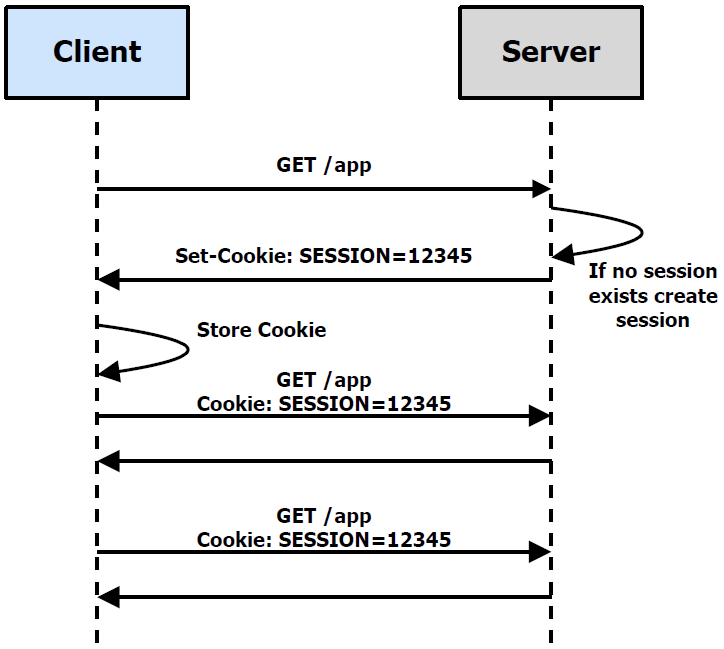
\includegraphics[width=0.6\textwidth]{./img/cookie-creation}
	\caption{Cookie Erzeugung über HTTP Request Header}
\end{figure}

\textbf{Cookie Attribute}
\begin{easylist}[itemize]
	& \textbf{Name=Content} (Key, value pair)
	&& Name: Cookie Name
	&& Content: Cookie Value
	&& Beispiel: jsessionid=klrezbxur234kls
	& \textbf{Domain} (domain=.google.com)
	&& Ort wohin das Cookie gesendet werden kann.
	&& Default: No domain: Cookie wird nur an den Server gesendet, von dem es stammt.
	& \textbf{Path} (path=/app)
	&& URL-Path wohin das Cookie gesendet werden kann.
	&& Default: No path: Cookie wird nur an den Pfad gesendet, von dem es stammt.
	& \textbf{Secure} (Secure (flag only))
	&& Cookie wird nur über HTTPS übermittelt.
	&& Default: insecure
	& \textbf{Expires} (expires: Sun, 17-Jan-2038 19:14:07 GMT)
	&& Gültigkeit des Cookies.
	&& Default: No date: Cookie wird nicht persistiert, nur Browsersession.
	& \textbf{HttpOnly} (HttpOnly (flag only))
	&& Auf Cookie kann nicht aus JavaScript Code zugegriffen werden.
	&& Default: nicht vorhanden: JavaScript kann mit document.cookie darauf zugreifen.
\end{easylist}

Wann ein Cookie \textbf{an den Server gesendet} wird, ist abhängig von mehreren Attributen: Domain, Path, Secure und Expire.\\
Das HttpOnly Attribut bietet einen Schutz vor XSS, wobei es JavaScript Code, welcher eingeschleust wurde, verbietet, auf das Cookie zuzugreifen.

Beispiel: Temporäres Cookie (non-persistent), dass nur per HTTPS zur Ursprungsseite übertragen wird:
\textit{Set-Cookie: SESSION=123; path=/app; Secure; HTTPOnly}

\subsubsection{SSL Session ID}
Mithilfe der \textit{SSL Session ID} können SSL-Sessions weiter verwendet werden, ohne einen erneuten Handshake durchzuführen. Ähnlich wie bei Cookies werden diese zu beginn der Anfrage an den Server übermittelt, welcher den zur ID passenden symmetrischen Schlüssel besitzt.\\
Der gesamte Payload des SSL-Pakets ist verschlüsselt, man sieht also weder die URL noch andere Inhalte des HTTP-Pakets.

\subsection{Angriffsszenarien}
Nebst der bereits erwähnten \textbf{Back Button Relogin Vulnerability} existieren noch weitere gängige Angriffsszenarien.

\subsubsection{Session Fixation}
Bei einer Session Fixation Attacke erzeugt der Hacker bei der verwundbaren Webseite eine Session (ohne Login). Diese Session wird nun dem Opfer mit einem Link mitgeteilt. Das Opfer authentifiziert sich auf der Webseite unter Verwendung dieser Session und ermöglicht es somit dem Hacker, die authentifizierte Session zu benützen.

Abwehrmassnahmen:
\begin{easylist}[itemize]
	& Neue Session erzeugen nach erfolgreicher Authentifizierung
	& Cookies verwenden, um die SessionID zu speichern
	& Cookies mit den entsprechenden Attributen sichern
\end{easylist}

\subsubsection{SQL Injection}
Der Angreifer versucht dabei, über die Anwendung, die den Zugriff auf die Datenbank bereitstellt, eigene Datenbankbefehle einzuschleusen. Dies wird durch Sicherheitslücken ermöglicht, die durch \textbf{mangelnde Maskierung oder Überprüfung von Metazeichen in Benutzereingaben} entstehen. Solche Schwachstellen sind im Code leicht zu erkennen, beim Testen jedoch nicht mehr.
Beispiele
\begin{easylist}[itemize]
	& SELECT * FROM Users WHERE Username='\textcolor{red}{Muster}' AND Password='\textcolor{red}{'OR''='}'
	& SELECT 1, 2, 3 FROM Employees WHERE City='\textcolor{red}{'UNION ALL SELECT OtherField, '', '' FROM OtherTable WHERE ''='}'
\end{easylist}

\textbf{Time Based Blind SQL Injection}\\
SQL Injection, bei der man keine Fehlermeldung sieht aber anhand der Antwortzeit auswertet, ob es sich um einen erfolgreichen Angriff handelt oder nicht. Die Antwortzeit kann durch \textbf{datenbankinterne Benchmark-Funktionen} verlängert werden.\\

\textbf{Gegenmassnahmen}\\
Als Gegenmassnahme sollte \textbf{in erster Priorität das Problem im Sourcecode behoben werden}. Anschliessend kann als generellen Schutz eine WAF (Web Application Firewall) vorgeschaltet werden und der mögliche Schaden durch hardening des DB-Servers weiter eingegrenzt werden.

\begin{description}
	\item[Secure Programming] Prepared Statements (Java), Parameters Collections (.NET), Stored Procedures (DB), Proper Error Handling, no plaintext passwords in database
	\item[Second Line of Defense] WAF, Input Validation, Encoding \item[Database Hardening] pro Datenbank eine DB-Instanz, Administrator Account nicht für Applikations-Zugriff verwenden, Default Admin Accounts deaktivieren, mehrere Benutzer für verschiedene Module der Applikation, restriktive Berechtigungen (\textit{Principle of least privilege}), Views für Read-Only
\end{description}

\subsubsection{Cross Site Scripting - XSS}
Die Gefahr für XSS entsteht, wenn Benutzereingaben unzureichend gefiltert werden und unverändert wieder an andere Benutzer ausgeliefert werden. Dies ermöglicht z.B. die Übernahme von Sessions, HTML- oder JS-Injection, Exploit injection oder Keylogging.\\
Es werden drei Typen von Attacken unterschieden:
\begin{description}
	\item[Stored] Das injizierte Skript ist permanent auf dem Zielserver gespeichert, z.B. in Form von Forumsbeiträgen.
	\item[Reflected] Das Skript wird nicht auf dem Zielserver gespeichert, der Angreifer muss aber eine URL präparieren und diese dem Opfer unterjubeln. Dies ist z.B. über eine Suchanfrage möglich.
	\item[DOM based] Angreifer muss eine URL präparieren, welche dann im Client direkt ausgelöst wird. Server wird dabei nicht aufgerufen, clientseitige Validierung nötig.
\end{description}

Mögliche \textbf{Gegenmassnahmen} sind:
\begin{description}
	\item[HTML entities] Encoding vor dem Speichern und bei der Ausgabe.
	\item[Client Security] X-XSS-Protection
	\item[HTTP Only Cookies] Auslesen über JS nicht möglich.
	\item[CSP] Content Security Policy: \lstinline|script-src 'self'|
\end{description}

\subsubsection{JSON-Hijacking}
JSON-Hijacking zielt darauf ab, sensitive Daten, die in JSON Format an einen authentifizierten Empfänger übermittelt werden, zu stehlen. Dabei präpariert der Angreifer eine Seite mit einem JavaScript, welches die Callback-Funktion, den \textit{Property Setter} oder den \textit{Array-Constructor} überschreibt. Als zweites wird ein GET Request auf die verwundbare Seite durchgeführt. Die Response kann dann vom Angreifer verarbeitet und die Daten gespeichert werden.\\

\textbf{Lösung:}
\begin{easylist}
	& Token in Request URLs verwenden, sodass diese nicht erraten werden können
	& JSON Response mit einem Infinite Loop beginnen
	& JSONP vermeiden (JSONP-Aufrufe sind \textbf{immer verwundbar} für JSON-Hijacking)
	& Arrays in ein JSON-Objekt einbetten
\end{easylist}

\subsubsection{Clickjacking-Attacke}
Dabei wird dem Opfer ein Frame über einen anderen Inhalt gelegt und so versucht, durch Klicken Aktionen auf dem dahinter liegenden Objekt auszuführen.\\
Gegenmassnahme: Die \textbf{X-Frame-Options} im HTTP Response Header kann verwendet werden, um zu bestimmen, ob ein aufrufender Browser die Zielseite in einem \lstinline|<frame>|, \lstinline|<iframe>| oder \lstinline|<object>| rendern darf. Webseiten können so unterbinden, dass ihr Content in fremden Seiten eingebettet wird.
\textbf{CSP hat Vorrang} vor X-Frame-Headers, weil die Unterbindung von Frames seit Version 2.0 dort auch integriert ist.

\begin{lstlisting}[caption=Clickjacking mittels X-Frame-Options unterbinden, language={}]
X-Frame-Options: DENY [SAMEORIGIN, ALLOW-FROM https://example.com/]
\end{lstlisting}

\subsection{Sicherheitskonzepte}

\subsubsection{Same Origin Policy}
Damit wird im Browser verhindert, dass clientseitiger Script-Code von einer Website auf DOM und Cookies einer anderen Website zugreifen kann. Nur bei Übereinstimmung der \textbf{Origin}, also gleichem \textbf{Protokoll, Hostname und Port}, wird dies erlaubt.\\
Folgende Scripts werden von der SOP behandelt:
\begin{easylist}[itemize]
	& JavaScript
	& XMLHttpRequest (XHR), XDomainRequest (XDR)
	& Java Applet, Adobe Flash, Microsoft Silverlight, ActiveX
	& Browser Extensions und Plugins
\end{easylist}
Wird nun aber in der Ursprungs-Seite ein 3rd-Party-Script durch \lstinline|<script src="...">| geladen, so kann es auf Cookies der Ursprungs-Seite zugreifen.\\
Die Übermittlung von Daten an fremde Seiten kann dann über Bild-Tags erfolgen, da diese nicht der SOP unterliegen.\\
Wird der Javascript-Code über die URL injiziert, so spricht man von \textbf{Reflected XSS}. Der XSS-Schutz im Browser kann dies verhindern, aber nicht bei \textbf{Stored XSS}.

\subsubsection{Cross Origin Resource Sharing - CORS}
Dies ist eine mögliche Aufweichung der SOP, denn manchmal ist gerade eine Cross-Domain-Kommunikation zwingend erforderlich.
Damit schützt sich beispielsweise ein Service-Anbieter (z.B. Google-API), welcher seine Daten ausschliesslich für berechtigte Nutzer oder weitere eigene Domains (z.B. youtube.com) zur Verfügung stellen möchte.\\
Anfragen an den Service Provider enthalten einen Header \lstinline|Origin: http://foo.example.com|. Die Antwort darauf den Header \lstinline|Access-Control-Allow-Origin: http://foo.example.com| (Es sind auch Wildcards möglich).\\

\textbf{CORS Preflighted Request}\\
Im Gegensatz zur simplen Anfrage wird beim Preflighted Request zuerst über einen HTTP-OPTIONS-Request abgefragt, ob der eigentliche Request sicher gesendet werden kann. Dies wird bei Anfragen gemacht, auf die eine der folgenden Bedingungen zutrifft:
\begin{easylist}[itemize]
	& Verwendung einer Methode ausser GET, HEAD oder POST.
	& POST fordert Daten mit einem anderen Content-Type als \lstinline|application/x-www-form-urlencoded|, \lstinline|multipart/form-data| oder \lstinline|text/xml| an
	& POST sendet Daten mit einem XML-Payload zum Server.
\end{easylist}

\begin{figure}[H]
	\centering
	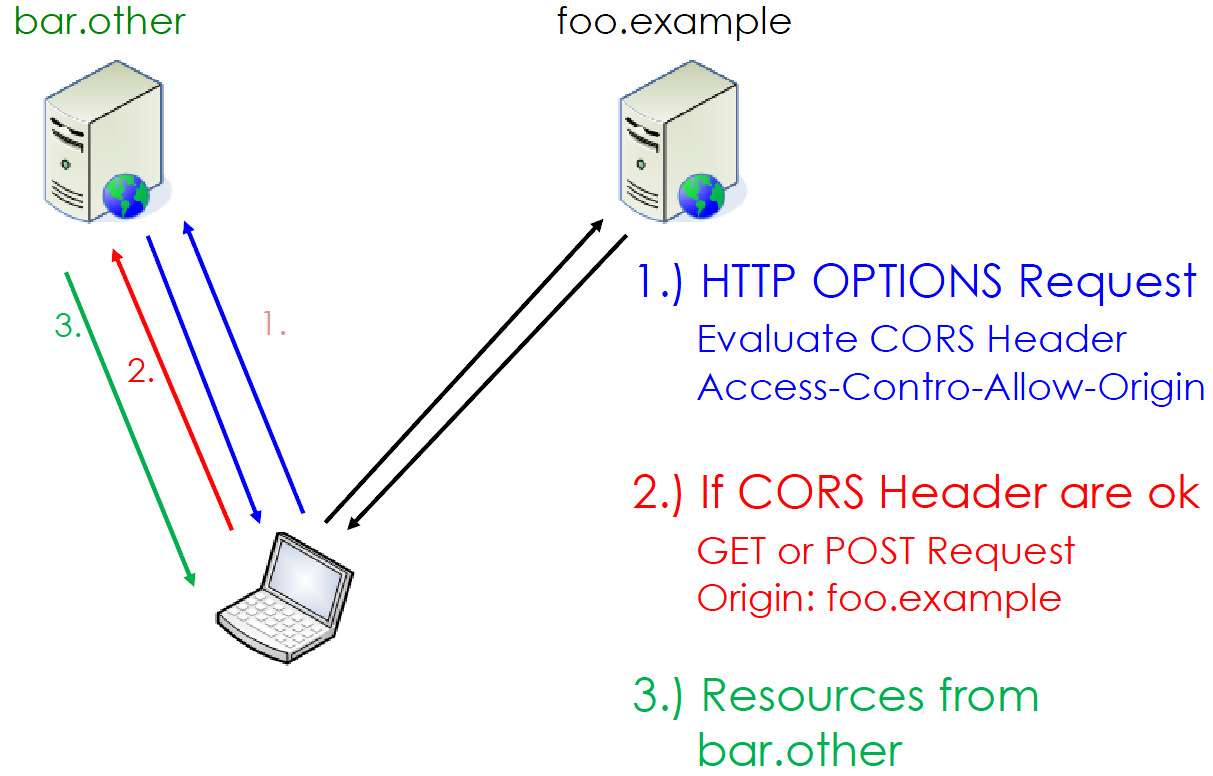
\includegraphics[width=0.6\textwidth]{./img/cors-preflight}
	\caption{Vorgehen beim CORS Preflight}
\end{figure}

Standardmässig werden bei Cross-Site-XMLHttpRequests-Aufrufen keine Credentials (Cookies) mitgeschickt. Um dies zu forcieren, muss ein spezielles Flag (\lstinline|xmlHttp.withCredentials|) auf dem Request-Objekt gesetzt werden.

\subsubsection{Content Security Policy - CSP}
CSP ist ein Sicherheitsstandard, der XSS, Clickjacking und weitere Code-Injection-Attacken verhindern soll. Dabei kann im Server konfiguriert werden, von welcher Origin Content (scripts, images, etc.) geladen werden darf. Treffen auf ein Element mehrere CSPs zu, wird immer die restriktivste benutzt.\\
CSPs können als HTTP-Response-Header-Feld \textit{Content-Security-Policy} (bei IE 10+ \textit{X-Content-Security-Policy}) oder im HTML Meta Element \lstinline|<meta http-equiv="X-Content-Security-Policy">| definiert werden.

\begin{lstlisting}[caption=Starter Policy für CSP-Header, language={}]
Content-Security-Policy: default-src 'none'; script-src 'self'; connect-src 'self'; img-src 'self'; style-src 'self';
\end{lstlisting}

Das Vorgehen beim Erstellen einer neuen CSP ist wie folgt:
\begin{enumerate}
	\item CSP-Header bei allen Requests hinzufügen mit Policy \lstinline[language=clean]|default-src 'none'|
	\item Verstösse in der Browser-Konsole anschauen
	\item Nötige Quellen zur Policy hinzufügen
\end{enumerate}

CSP hat folgende Defaults aktiviert:
\begin{enumerate}
	\item Keine Inline Javascript-Snippets. Nur aus Files 
	\item Keine JS-URLs wie javascript:http://url
	\item Eventhandling-Attribute sind deaktiviert (zum Beispiel document.click())
	\item Funktion eval() ist deaktiviert
	\item Der Konstruktor von function() ist deaktiviert
	\item URIs sind nur für Bilder erlaubt
\end{enumerate}

\subsubsection{X-XSS-Protection}
Dieser Header aktiviert den XSS-Schutz im Browser, jedoch kann dieser \textbf{nur Reflected XSS} erkennen. Bisher wird es nur von IE, Chrome und Safari unterstützt. In diesen Browsern sollte er jedoch standardmässig aktiviert sein.

\begin{lstlisting}[language={},caption=Beispiel des X-XSS-Protection Headers]
X-XSS-Protection: 1; mode=block
\end{lstlisting}

\subsection{SSL / TLS Verschlüsselung}

\subsubsection{Perfect Forward Secrecy - PFS}
Wenn zuvor ausgetauschte Langzeitschlüssel verwendet werden, um für jede zu verschlüsselnde Sitzung einen neuen geheimen Sitzungsschlüssel zu vereinbaren. Ein Protokoll hat \textit{Perfect Forward Secrecy}, wenn die verwendeten Sitzungsschlüssel nach Beendigung der Sitzung nicht mehr aus den geheimen Langzeitschlüsseln rekonstruiert werden können. Damit kann eine aufgezeichnete verschlüsselte Kommunikation auch bei Kenntnis des Langzeitschlüssels nicht nachträglich entschlüsselt werden.

\subsubsection{HTTP Strict Transport Security - HSTS}
Ein Sicherheitsmechanismus für HTTPS-Verbindungen. Er soll vor Aushebelung der Verbindungsverschlüsselung durch eine Downgrade-Attacke (z.B. \textit{sslstrip}) und vor Session Hijacking schützen. Durch die Angabe eines Header-Felds mit Hilfe von \textbf{mod\_headers} wird jede weitere Verbindung bis zum Erreichen der \textit{max-age} als \textbf{HTTPS erzwungen}, auch wenn ein Request oder die Seite selbst HTTP festlegen. Zusätzlich wird eine Verbindung mit dem Server unterbunden, sobald \textbf{Zertifikats-Probleme} auftauchen.\\

Google Chrome, wie auch andere Browser verwenden \textbf{HSTS-Preload-Listen}. Damit wird die Limitierung des \textit{trust on first use}-Prinzip für eine definierte Liste von Domains umgangen.

\begin{lstlisting}[language={},caption=HSTS-Header mit einer max-age von 30 Tagen]
Strict-Transport-Security: max-age=2592000 [; includeSubdomains]
\end{lstlisting}

\textbf{Bypassing HSTS}\\
HSTS ist Zeit-basiert (\textit{NTP}) und wird für eine gewisse Zeitspanne definiert. Um dies zu umgehen, wird die aktuelle Zeit geändert, wodurch das HSTS abläuft und der Browser ohne Warnung auf einen Fake-Server zugreift.

\subsubsection{HTTP Public Key Pinning - HPKP}
Der Browser erhält von der besuchten Website eine Liste mit allen gültigen Public Keys und speichert diese lokal ab. Wird bei einer späteren Verbindung ein Schlüssel verwendet, der nicht in dieser Liste ist, erscheint dem Benutzer eine Fehlermeldung, die nicht (leicht) zu umgehen ist. So sollen Man-in-the-Middle-Angriffe mit gefälschten Zertifikaten vermieden werden.\\

Google Chrome wie auch Firefox verwenden \textbf{Preload-Listen}. Damit wird die Limitierung des \textit{trust on first use}-Prinzip für eine definierte Liste von Domains umgangen.

\begin{lstlisting}[language={},caption=Beispiel des HPKP-Headers]
Public-Key-Pins: pin-sha256="base64=="; max-age=expireTime [; includeSubdomains][; report-uri="reportURI"]
\end{lstlisting}

\subsubsection{Certificate Revocation}
Wird der Private Key eines Zertifikats gestohlen oder "'geknackt"', so muss es natürlich als ungültig erklärt werden. Dies geschieht über die \textbf{Certificate Revocation List (CRL)}, die durch die \textit{Certificate Authority (CA)} verwaltet wird, welche bereits das Zertifikat ausgestellt hat. Die URL zur CRL ist Teil des Server-Zertifikats.\\

Der Eintrag in der CRL kann mit Hilfe des \textbf{Online Certificate Status Protocol (OCSP)} abgefragt werden. \textbf{Dies sollte vor jeder Verwendung eines Zertifikats automatisch gemacht werden.}

\subsubsection{Mutual Authentication / Two-Way Authentication}
Dies ist theoretisch ein absoluter Schutz gegen \textit{Man-in-the-Middle-Angriffe}, wird in der Praxis aber selten eingesetzt, da die Benutzerfreundlichkeit darunter leidet.
Nebst dem Server-Zertifikat muss nun auch der Client ein Zertifikat bereitstellen, das der Server überprüfen kann. Durch diese zweifache Authentifizierung ist ein MITM-Angriff, zumindest im Network-Layer, ausgeschlossen.

\begin{figure}[H]
	\centering
	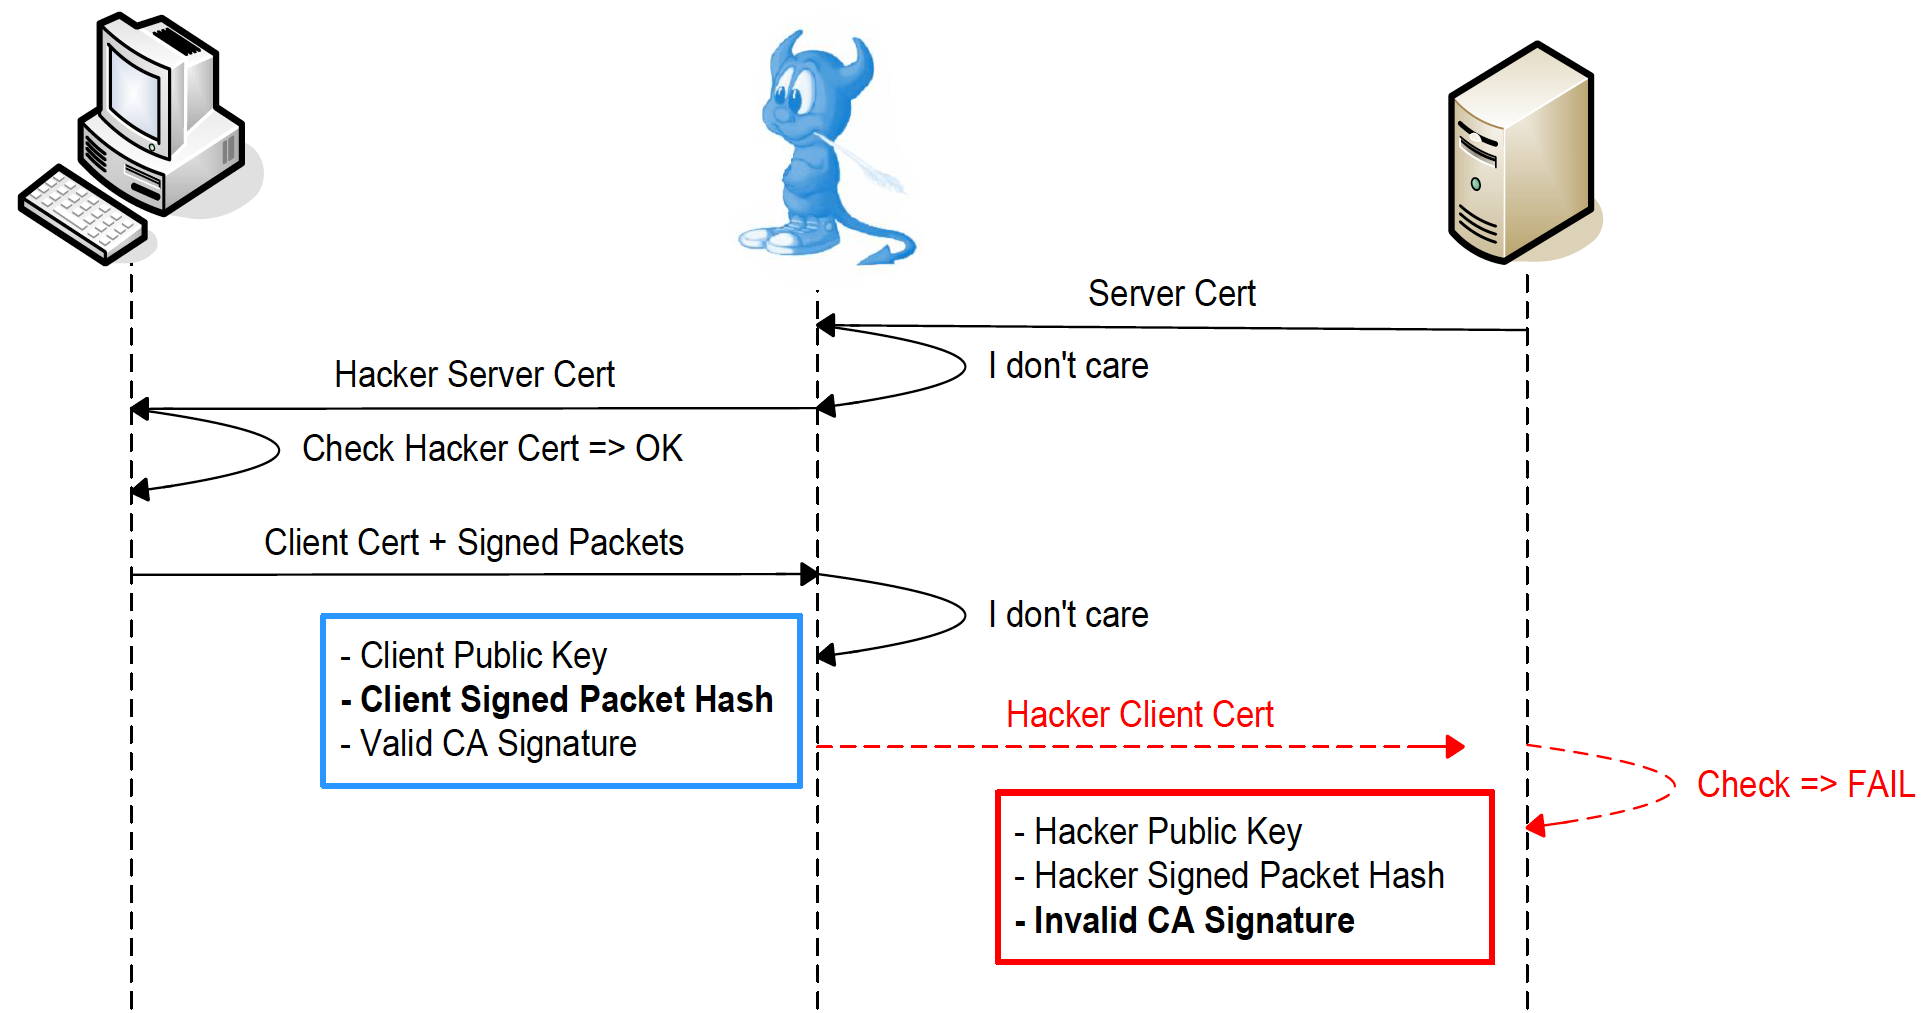
\includegraphics[width=\textwidth]{./img/mutual-authentication}
	\caption{Beispielablauf eines fehlgeschlagenen Man-in-the-Middle-Angriffs}
\end{figure}